\documentclass{article}

\usepackage[italian]{babel}
\usepackage[utf8]{inputenc}
\usepackage{hyperref}
\usepackage{natbib}
\usepackage{graphicx}
\usepackage{float}
\usepackage[margin=2.5cm]{geometry}
\usepackage{wrapfig}
\usepackage{minted}

\title{ATTSW Exam}
\author{Gabriele Puliti - \texttt{5300140} - \href{mailto:gabriele.puliti@stud.unifi.it}{\textit{gabriele.puliti@stud.unifi.it}}}
\date{December 2017}

\begin{document}

\maketitle

\begin{flushleft}

% https://docs.gradle.org/current/userguide/userguide.html

\section{Gradle} % https://github.com/gradle/gradle 
Gradle è un progetto open source che fornisce un tool di build automation, che può essere un ottimo sostituto di Maven. Offre un modello in grado di supportare l'intero ciclo di vita dello sviluppo del software ed è stato progettato per supportare build automation attraverso più linguaggi e piattaforme. Nel nostro caso considereremo questo tool per lo sviluppo di software Java.


\subsection{Differenze tra Gradle e Maven} % https://gradle.org/maven-vs-gradle/
Ci sono molte differenze tra questi due tools: flessibilità, performance, gestione delle dipendenze e molto altro. La configurazione di Gradle di un progetto ha una convenzione molto più facile e comprensibile rispetto alla tediosa e a volte impossibile configurazione del pom.xml di Maven. Entrambi usano dei metodi di miglioramento della velocità di esecuzione delle build. Gradle infatti evita il lavoro di monitoraggio dei task di I/O eseguendo solo il necessario e quando possibile processare solo i files che sono cambiati (incrementality). Utilizza anche un sistema di cache riusando gli outputs di altre build Gradle con gli stessi inputs (Build Cache). Sfrutta anche un long-lived process che mantiene tutte le informazioni in memoria (Gradle Deamon). Queste 3 caratteristiche rendono Gradle molto veloce, una build eseguita con Gradle con Maven verrebbe completata con un tempo 3 volte maggiore. Tutto questo è anche possibile grazie a un sistema di esecuzioni parallele di task e intra-task.
\begin{figure}[H]
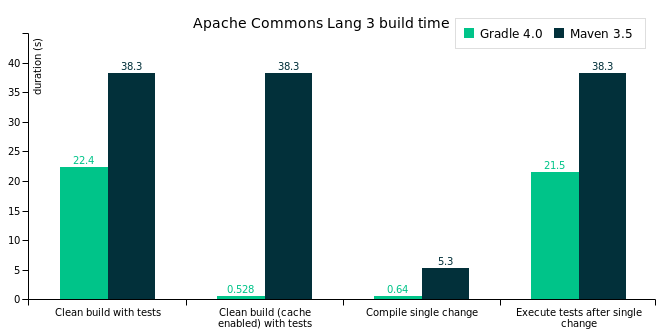
\includegraphics[scale=0.70]{performance.png}
\end{figure} 
% https://docs.gradle.org/current/userguide/userguide.html


\subsection{Installazione}
L'istallazione di Gradle può essere fatta in più modi: tramite installazione manuale o utilizzando un package manager (tutte le informazioni possono essere trovate in \textbf{\href{https://gradle.org/install/}{questo link}}). Personalmente consiglio l'utilizzo del software development kit manager \textbf{\href{http://sdkman.io/}{SDKMAN!}} che non solo permette l'installazione molto facilitata di Gradle, ma anche della JVM e di tanti altri tools.

\subsubsection{installazione tramite SDKMAN!}
L'installazione si basa su 2 semplici comandi:
\begin{verbatim}
  $ curl -s "https://get.sdkman.io" | bash
  
  $ source "$HOME/.sdkman/bin/sdkman-init.sh"
\end{verbatim}
A questo punto se tutto è andato a buon fine SDKMAN! è stato installato correttamente, è possibile verificarlo digitando il comando su terminale:
\begin{verbatim}
  $ sdk version
\end{verbatim}
l'output risultante dovrebbe essere qualcosa del tipo:
\begin{verbatim}
  SDKMAN 5.5.15+284
\end{verbatim}
Ora è possibile procedere con l'installazione di Gradle. Prima di tutto visualizziamo la lista delle versioni di Gradle:
\begin{verbatim}
  $ sdk list gradle
\end{verbatim}
L'output corrispondente sarà:
\begin{verbatim}
================================================================================
Available Gradle Versions
================================================================================
     4.4.1                4.2-rc-2             3.0                  2.10           
     4.4-rc-6             4.2-rc-1             2.9                  2.1            
     4.4-rc-5             4.2                  2.8                  2.0            
     4.4-rc-4             4.1                  2.7                  1.9            
     4.4-rc-3             4.0.2                2.6                  1.8            
     4.4-rc-2             4.0.1                2.5                  1.7            
     4.4-rc-1             4.0                  2.4                  1.6            
     4.4                  3.5.1                2.3                  1.5            
     4.3.1                3.5                  2.2.1                1.4            
     4.3-rc-4             3.4.1                2.2                  1.3            
     4.3-rc-3             3.4                  2.14.1               1.2            
     4.3-rc-2             3.3                  2.14                 1.12           
     4.3-rc-1             3.2.1                2.13                 1.11           
     4.3                  3.2                  2.12                 1.10           
     4.2.1                3.1                  2.11                 1.1            
================================================================================
+ - local version
* - installed
> - currently in use
================================================================================
\end{verbatim}
La versione che vogliamo installare è quella più recente che in questo caso è la 4.4.1, possiamo quindi eseguire il comando:
\begin{verbatim}
  $ sdk install gradle 4.4.1
\end{verbatim}
appena il download e l'installazione sarà finita possiamo verificare il completamento tramite:
\begin{verbatim}
  $ gradle -v
\end{verbatim}
che non solo stamperà su terminale la versione di Gradle, ma anche:
\begin{itemize}
  \item Groovy (libreria usata per i file di configurazione delle build)
  \item Ant (software usato per le build delle Java applications)
  \item Java Virtual Machine
  \item sistema operativo in uso
\end{itemize}
se l'output ha queste informazioni allora Gradle è stato completamente installato. SDKMAN! si preoccupa anche di creare la variabile \$GRADLE\_HOME che è possibile visualizzare con il comando \begin{verbatim} $ echo $GRADLE_HOME \end{verbatim} Se ci sono errori di tipo Java, i problemi possono essere:
\begin{itemize}
  \item Gradle non riesce a trovare la jdk, problema risolvibile installando java con sdkman con il comando \begin{verbatim}  $ sdk install java <versione> \end{verbatim}
  \item Java è aggiornato alla versione 9 o superiori (infatti attualmente Gradle non è aggiornato per versioni superiori alla 8), basterà fare un downgrade ad una versione precedente (possibile farlo anche tramite SDKMAN!).
\end{itemize}
In entrambi i casi sarà necessario anche comunicare al sistema la versione da usare: \begin{verbatim}  $ sdk use java <versione_installata> \end{verbatim} per essere sicuri che è stato installata la giusta versione di java possiamo controllare gli outputs dei seguenti comandi:
\begin{itemize}
  \item \begin{verbatim}  $ echo $JAVA_HOME \end{verbatim}
  \item \begin{verbatim}  $ java -version \end{verbatim}
\end{itemize}
il primo comando dovrà restituire in output il giusto percorso della JVM installata, il secondo serve a controllare la versione java attualmente in uso.


\section{Tutorial} % https://docs.gradle.org/current/userguide/tutorial_gradle_command_line.html
Propongo nei seguenti paragrafi alcuni esempi.

\subsection{Primo tutorial: gestione dei task}

\subsubsection{Task e Task dependency}
Come in Maven ci sono i goals in Gradle ci sono i task, ogni task ha il suo scopo che viene definito nella sua implementazione. Gradle si basa su build multi-task, il primo esempio si basa sulla comprensione del funzionamento delle build maven. Creiamo una cartella in cui inserire il file di configurazione della build Gradle chiamato build.gradle e modifichiamo il suo contenuto usando un editor di testo:
\begin{verbatim}
task compile {
    doLast {
        println 'compiling source'
    }
}

task compileTest(dependsOn: compile) {
    doLast {
        println 'compiling unit tests'
    }
}

task test(dependsOn: [compile, compileTest]) {
    doLast {
        println 'running unit tests'
    }
}

task dist(dependsOn: [compile, test]) {
    doLast {
        println 'building the distribution'
    }
}
\end{verbatim}
a questo punto dovremmo avere una cosa di questo tipo:
\begin{figure}[H]
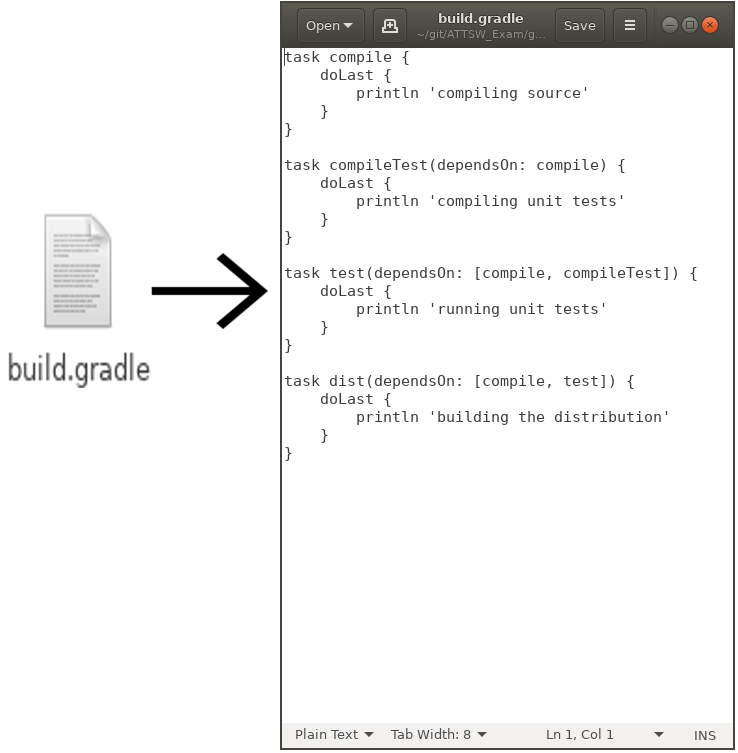
\includegraphics[scale=0.40]{gradleexamplefirst.png}
\end{figure} 
abbiamo creato un albero di dipendenze tra task di questo tipo:
\label{taskdip}
\begin{figure}[H]

\includegraphics[scale=0.70]{taskdipendence.png}
\end{figure} 
è possibile fare diverse build con questa configurazione:
\begin{itemize}
    \item \begin{verbatim} $ gradle compile \end{verbatim}
    \item \begin{verbatim} $ gradle compileTest \end{verbatim}
    \item \begin{verbatim} $ gradle test \end{verbatim}
    \item \begin{verbatim} $ gradle dist \end{verbatim}
    \item una combinazione qualunque di 2 o più task.
\end{itemize}
Possiamo notare che anche se facciamo la build: \begin{verbatim} $ gradle compile test \end{verbatim} il task \textbf{compile} verrà eseguito solo una volta:
\begin{verbatim}
> Task :compile 
compiling source

> Task :compileTest 
compiling unit tests

> Task :test 
running unit tests


BUILD SUCCESSFUL in 0s
3 actionable tasks: 3 executed
\end{verbatim}
\subsubsection{Escludere i task da una build}
È possibile escludere un task da una build in cui quel task verrebbe eseguito aggiungendo come argomento il task da escludere preceduto da -x:
\begin{verbatim}
    $ gradle <task_da_eseguire> -x <task_da_escludere>
\end{verbatim}
questo viene usato per evitare di eseguire un task inutile per lo scopo della build che vogliamo fare. Riprendendo l'esempio del paragrafo precedente se andiamo ad eseguire la build:
\begin{verbatim}
    $ gradle dist    
\end{verbatim}
vediamo che vengono eseguiti tutti i task, compresi i task \textbf{test} e \textbf{compileTest}, supponendo di voler fare solo la build del sorgente possiamo scrivere:
\begin{verbatim}
    $ gradle dist -x test
\end{verbatim}
l'output risultante sarà:
\begin{verbatim}
> Task :compile 
compiling source

> Task :dist 
building the distribution


BUILD SUCCESSFUL in 0s
2 actionable tasks: 2 executed
\end{verbatim}
Il task \textbf{compileTest} non viene eseguito perchè dipendenza di \textbf{test}, ma non di \textbf{dist} (vedi pag. \pageref{taskdip}), escludendo il primo quindi non è necessario eseguire il task \textbf{compileTest}.

\subsubsection{Approfondimenti}
I comandi eseguibili sono svariati:
\begin{itemize}
    \item \textbf{Abbreviazione del nome del task:} è possibile abbreviare il nome del task da eseguire stando però attenti a identificare unicamente il task che vogliamo eseguire, per esempio se volessi eseguire il task \textbf{compileTest} posso farlo semplicemente con il comando:
    \begin{verbatim}
    $ gradle comTes
    \end{verbatim}
    considerando i task creati precedentemente notiamo che il task è univocamente identificato.
    \item \textbf{Selezionare la build da eseguire:} consideriamo che esista in una subdirectory chiamata subdir una build chiamata subbild.gradle, partendo dalla directory root è possibile eseguire questa build eseguendo il comando:
    \begin{verbatim}
    $ gradle -b subdir/subbuild.gradle <task_da_eseguire>
    \end{verbatim}
    è possibile anche indicare direttamente la project directory da usare, nel nostro caso indicheremo subdir:
    \begin{verbatim}
    $ gradle -p subdir
    \end{verbatim}
\end{itemize}

% https://docs.gradle.org/current/userguide/tutorial_gradle_command_line.html#sec:rerun_tasks

\end{flushleft}
\end{document}
